\documentclass{ieeeaccess}
\usepackage{cite}
\usepackage{amsmath,amssymb,amsfonts}
\usepackage{algorithmic}
\usepackage{graphicx}
\graphicspath{{figures/}}
\usepackage{textcomp}
\usepackage{bm}
\usepackage{siunitx}
\usepackage{booktabs}

% --- Unicode character support (avoid compile errors with pdfLaTeX)
\DeclareUnicodeCharacter{0394}{\ensuremath{\Delta}}
\DeclareUnicodeCharacter{2265}{\ensuremath{\ge}}

% --- Bold math setup from template (kept as-is)
\makeatletter
\AtBeginDocument{\DeclareMathVersion{bold}
\SetSymbolFont{operators}{bold}{T1}{times}{b}{n}
\SetSymbolFont{NewLetters}{bold}{T1}{times}{b}{it}
\SetMathAlphabet{\mathrm}{bold}{T1}{times}{b}{n}
\SetMathAlphabet{\mathit}{bold}{T1}{times}{b}{it}
\SetMathAlphabet{\mathbf}{bold}{T1}{times}{b}{n}
\SetMathAlphabet{\mathtt}{bold}{OT1}{pcr}{b}{n}
\SetSymbolFont{symbols}{bold}{OMS}{cmsy}{b}{n}
\renewcommand\boldmath{\@nomath\boldmath\mathversion{bold}}}
\makeatother

\def\BibTeX{{\rm B\kern-.05em{\sc i\kern-.025em b}\kern-.08em
    T\kern-.1667em\lower.7ex\hbox{E}\kern-.125emX}}

\begin{document}

% --- Metadata placeholders (edit as needed)
\history{Submitted xxxx xx, 2026; revised xxxx xx, 2026; accepted xxxx xx, 2026.}
\doi{10.1109/ACCESS.20xx.xxxxxxx}

% --- Title / Authors (PLEASE UPDATE)
\title{A Time-Aware Evaluation Framework for Real-Time GPS Spoofing Detection in UAV-Based Power System Monitoring}
\author{\uppercase{Bingye Zhang}\authorrefmark{1},
\uppercase{Qian Zhang}\authorrefmark{1},
\uppercase{Xueyan Wang}\authorrefmark{1},
\uppercase{Xiaotian Fu}\authorrefmark{1},
\uppercase{Huaxi Luo}\authorrefmark{1},
\uppercase{Tao Qiu}\authorrefmark{2}}

\address[1]{State Grid Taizhou Power Supply Company, No. 809, Zhongxing Road, Jiaojiang District, Taizhou 318000, China}
\address[2]{Ningbo Induschain Digital Technology Co., Ltd., No. 161 Yongshuiqiao Road, Building 2, 18–19F, Haishu District, Ningbo 315000, China}

\tfootnote{This work was supported by Hongchuang Technology Branch 2025 Research on Network Security Testing and Protection Verification Technology Based on Transmission, Transformation, and Distribution UAVs, 521184250002}

\markboth{IEEE Access, Vol. xx, No. xx, Month 2026}
{Author \headeretal: A Time-Aware Evaluation Framework for Real-Time GPS Spoofing Detection in UAV-Based Power System Monitoring}

\corresp{Corresponding author: Xueyan Wang (e-mail: WXY421202@163.com).}

\begin{abstract}
Conventional evaluation metrics for UAV GNSS spoofing detection (e.g., precision
and recall) are static snapshot measures that do not quantify \emph{when} a threat
is detected or how frequently false alarms disrupt operations. This paper proposes
a \textbf{Time-Aware Evaluation Framework} that introduces three metrics aligned
with real deployment requirements: DR@$\Delta t$ (detection rate within a time
budget), ADD (average detection delay), and MTBFA (mean time between false alarms
with event-level aggregation). Thresholds are derived from UAV power-line
inspection risk: at 5 m/s cruise speed, a 5-second detection budget leaves
20 m of abort margin relative to the GB\,26860-2011 safe-approach distance.
Using 3\,000 MATLAB UAV Toolbox flights as the primary dataset (train-only
augmentation; strictly isolated test split) and zero-shot cross-domain evaluation
on real-world hardware datasets, we evaluate seven representative deep-learning
detectors as a case study of the framework's discriminative power. Results show
that the time-aware framework reveals risk-identification gaps that conventional
metrics consistently miss: models achieving $\geq$85\% precision may still fail to
detect the majority of attacks within the 5-second safety budget, or generate false
alarms at rates far below the operational tolerance. All results are reported as
mean $\pm$ 95\% confidence interval over 5 random seeds with Bonferroni-corrected
significance testing. The framework is detector-agnostic and portable to other
event-detection domains.
\end{abstract}

\begin{keywords}
Time-aware evaluation, GNSS/GPS spoofing detection, UAV security, real-time detection, deep learning, false alarms.
\end{keywords}

\titlepgskip=-21pt
\maketitle

\section{Introduction}

With the widespread adoption of unmanned aerial vehicles (UAVs) in power-system inspection and related applications, UAV navigation and positioning increasingly depend on global navigation satellite systems (GNSS/GPS) \cite{ref1}. In low-redundancy scenarios where external aids such as LiDAR or visual SLAM are unavailable, GNSS often becomes the primary (and sometimes the only) source for self-localization and waypoint tracking \cite{ref2}. This heavy reliance exposes UAVs to severe navigation-security threats-most notably \textbf{GNSS spoofing attacks} \cite{ref3}. In spoofing, an attacker transmits forged satellite-like signals that mislead the UAV into accepting falsified position information \cite{ref4}. During power-line inspection, manipulated navigation can cause trajectory deviation, boundary violations, and dangerously close approaches to high-voltage assets, potentially resulting in collisions, crashes, and mission failures \cite{ref5}. Such incidents can endanger both infrastructure and the UAV platform and may lead to substantial economic losses \cite{ref6}.

To address these threats, industry and academia have increasingly studied UAV GNSS spoofing detection and explored deep-learning-based solutions. Borhani-Darian \textit{et al.} proposed a detection approach combining deep neural networks with clustering and demonstrated strong performance across different SNR conditions \cite{ref7}. Sun \textit{et al.} built a hybrid architecture integrating PCA, CNN, and LSTM and reported 99.49\% accuracy for GPS spoofing detection \cite{ref8}. Badar \textit{et al.} proposed a CNN-BiLSTM hybrid model and improved detection on imbalanced datasets via feature selection, achieving 99.25\% accuracy \cite{ref9}.

However, most existing work evaluates such detectors using conventional classification metrics such as \textbf{precision} and \textbf{recall}. While these static metrics capture offline classification quality, they are limited for practical deployment where \textbf{timeliness} and \textbf{false-alarm control} are critical. In other words, even a detector with high offline precision may be unsafe in real operations if it cannot raise alarms promptly or if it produces frequent false alarms.

The absence of an explicit time dimension prevents traditional metrics from quantifying dynamic properties such as response speed and false-alarm frequency. In intrusion detection systems (IDS), researchers have long recognized these limitations. Axelsson showed that IDS usability depends not only on detection rate but also on false-alarm rate; even 99\% detection becomes impractical with a 10\% false-alarm rate at scale \cite{ref10}. Sommer and Paxson further discussed the \textbf{base-rate fallacy}: in real environments where attacks are rare, even high-accuracy detectors can generate large numbers of false alarms due to the low base rate \cite{ref11}. These insights highlight how precision/recall can be misleading for imbalanced data, yet they still do not quantify detection delay.

In UAV navigation-security detection, evaluation remains dominated by conventional metrics. For example, Almadhor \textit{et al.} proposed the compact CTDNN-Spoof architecture and reported mainly accuracy and training time \cite{ref12}. A survey by Rehman Badar \textit{et al.} indicates that nearly all GNSS spoofing detection studies rely on precision and recall and severely lack quantification of time sensitivity, especially for false-alarm frequency and alert delay \cite{ref9}. Shafique \textit{et al.} reviewed more than 20 GNSS spoofing detection methods and found that almost all used accuracy/precision/recall; only three papers mentioned "detection time," and none provided a clear definition or systematic measurement \cite{ref13}.

Neglecting time factors can have serious operational consequences. Even if a detector is highly accurate offline, a long alarm delay may allow the UAV to drift hundreds of meters before detection-too late for safe intervention. Likewise, frequent false alarms can overwhelm operators and lead to \textbf{alarm fatigue} \cite{ref14}, causing alerts to be ignored and rendering the system ineffective, increasing the risk of accidents and economic loss. Therefore, relying solely on static metrics such as precision and recall is inadequate for real-time UAV navigation-security missions \cite{ref9}, \cite{ref15}.

Some real-time-focused domains have begun emphasizing detection speed. Panda and Guo proposed a Bayesian online changepoint detection (BOCPD) method that detects subtle spoofing-induced trajectory drift and significantly reduces recognition time \cite{ref16}. Dasgupta \textit{et al.} used reinforcement learning to detect GPS spoofing in autonomous navigation; their model can trigger timely alerts within maneuver intervals while maintaining high precision and recall \cite{ref17}. However, these works often define domain-specific temporal metrics and lack a general-purpose evaluation framework.

In time-series anomaly detection, Tatbul \textit{et al.} proposed \textbf{time-series-aware precision and recall}, incorporating temporal continuity of anomalies into evaluation \cite{ref18}. They argued that pointwise metrics overcount sustained anomalies: for instance, a 10-minute anomaly at 1 Hz marked continuously would produce 600 true positives, even though it should be counted as a single successfully detected event. Their event-level evaluation mitigates this distortion. Yet the framework mainly targets offline settings and does not model causality constraints or detection delay in online detection.

Motivated by these observations, we propose a \textbf{Time-Aware Evaluation Framework} for UAV GNSS spoofing detection. Without restricting the detector architecture, the framework introduces time-aware metrics that characterize \textbf{detection speed} and \textbf{false-alarm frequency}, bridging the gap between traditional metrics and deployment requirements. Concretely, our contributions are:

\begin{itemize}
\item \textbf{Formal online detection modeling}: We introduce the notion of \textbf{Discrete Decision Times} to formulate online detection as an event-detection problem with explicit temporal semantics and causality constraints.
\item \textbf{Time-aware metrics}: We propose three core metrics---\textbf{DR@$\Delta t$}, \textbf{ADD}, and \textbf{MTBFA}---to systematically quantify detection speed and false-alarm frequency.
\item \textbf{False-alarm event aggregation}: We model temporal continuity and aggregate consecutive false-positive windows into a single false-alarm event, aligning false-alarm frequency with operational burden.
\item \textbf{Systematic experimental validation}: Using 3\,000 MATLAB UAV Toolbox simulation flights as the primary dataset---with strictly isolated test splits and optional train-only augmentation---we evaluate seven representative deep-learning detectors as a case study and reveal consistent discrepancies between conventional and time-aware metrics, corroborated by zero-shot cross-domain evaluation on real-world hardware datasets.
\end{itemize}

The remainder of this paper is organized as follows. Section II defines the task and problem setup. Section III presents the proposed time-aware evaluation framework and metrics. Section IV describes the experimental design and implementation. Section V reports experimental results and analyses. Section VI concludes and discusses future work.

\section{Problem Setup}

\subsection{Online Detection Task and Scope}

We study UAV navigation security for waypoint-based power-line inspection missions. Under low-redundancy navigation conditions without LiDAR or visual SLAM, the UAV primarily relies on GNSS/GPS observations and onboard inertial/kinematic states (position, velocity, acceleration) to track its trajectory \cite{ref19}. An attacker can spoof GNSS observations so that the ground station and flight controller receive location information that deviates from the true motion state, causing trajectory drift, boundary violations near critical infrastructure, or mission failure \cite{ref20}.

Our core task is: given a time-ordered onboard navigation state sequence \(\{\mathbf{x}_t\}\) (feature dimension \(d\)), train an online binary detector \(f: \mathbb{R}^d \to \{0,1\}\) that outputs at each decision time whether the system is under spoofing attack, i.e., \(\hat{y}_{\tau_k} \in \{0,1\}\). The operational goal involves two coupled dimensions:

\begin{itemize}
\item \textbf{Timeliness}: once an attack starts, the system should trigger an alert as close as possible to the attack onset so that mitigation can be taken promptly (e.g., switching navigation sources, emergency return-to-home).
\item \textbf{False-alarm control}: during normal flight, false alarms should be minimized to reduce operational burden.
\end{itemize}

To make the notion of "online" reproducible in experiments, we define an attack as an event with a clear onset: the attack starts at time \(t_s\) and subsequently influences GNSS observations (duration is specified by the injection model; see Section IV-B). The ground-truth label can be expressed as

\begin{equation}
 y(t) = \mathbb{I}(t \ge t_s),
\end{equation}

where \(\mathbb{I}(\cdot)\) is the indicator function. Under this definition, key detector behavior is characterized by the \textbf{first alarm time} and the \textbf{detection delay}.

\subsection{Causality and Decision-Time Semantics}

Since the prediction made at time \(\tau_k\) can only depend on observations received up to \(\tau_k\) (and not on any future information), we introduce \textbf{Discrete Decision Times} to formalize causality.

We model online detection as producing predictions at a sequence of discrete times \(\{\tau_k\}_{k=1}^K\), where each \(\tau_k\) corresponds to a decision action. At decision time \(\tau_k\), the detector outputs a binary decision \(\hat{y}_{\tau_k}\) based only on observations up to \(\tau_k\).

Let the detector be a function \(f: \mathcal{X} \to \{0,1\}\) over an input space \(\mathcal{X}\) (e.g., fixed-length windows, variable-length sequences). At decision time \(\tau_k\), the detector receives input \(\mathbf{z}_k\) constructed from history and outputs

\begin{equation}
\hat{y}_{\tau_k} = f(\mathbf{z}_k).
\end{equation}

Define the first detection time (first positive after attack onset) and the attack onset time; then the detection delay is computed accordingly. A causal illustration of online detection is shown in Fig.~\ref{fig:causality}.

\begin{figure}[!t]
\centering
\includegraphics[width=\columnwidth]{fig_iii_1_causality.pdf}
\caption{Causality illustration for online detection.}
\label{fig:causality}
\end{figure}

\section{Proposed Time-Aware Evaluation Framework}

This section presents the proposed \textbf{Time-Aware Evaluation Framework} for online detection. The objective is to establish a detector-implementation-agnostic evaluation system that captures runtime properties---especially \textbf{detection speed} and \textbf{false-alarm frequency}---thereby bridging the gap between conventional classification metrics and deployment needs. Table~\ref{tab:notation} summarises all notation used throughout the framework.

% --- Notation table ---
\begin{table}[!t]
\caption{Summary of mathematical notation.}
\label{tab:notation}
\centering
\begin{tabular}{lll}
\toprule
\textbf{Symbol} & \textbf{Description} & \textbf{Unit} \\
\midrule
$k$          & Window index (decision step)          & --- \\
$\tau_k$     & Timestamp of the $k$-th window (end-point) & s \\
$t_s$        & Attack onset time                     & s \\
$t_d$        & First detection time after $t_s$      & s \\
$\delta_k = t_d - t_s$ & Detection delay             & s \\
$\Delta t$   & Detection time budget                 & s \\
$L$          & Window length (number of samples)     & samples \\
$S$          & Window stride (step size)             & samples \\
$f_s$        & Sensor sampling rate                  & Hz \\
$K$          & Number of windows per flight          & --- \\
$N$          & Total number of windows in a split    & --- \\
$F$          & Feature dimensionality (state vector) & --- \\
$\hat{y}_k \in \{0,1\}$ & Binary detector decision at step $k$ & --- \\
DR@$\Delta t$  & Detection rate at time budget $\Delta t$ & --- \\
ADD & Average detection delay               & s \\
MTBFA & Mean time between false alarms      & h \\
\bottomrule
\end{tabular}
\end{table}

\subsection{Discrete-Time Formulation of Online Detection}

We formalize the output of an online detector as a discrete-time sequence:

\begin{equation}
\mathcal{D} = \{(\tau_k, \hat{y}_{\tau_k})\}_{k=1}^K,
\end{equation}

where \(\tau_k\) is the timestamp of the \(k\)-th decision and \(\hat{y}_{\tau_k}\) is the corresponding binary decision. For notational convenience, we also write \(\hat{y}_k\triangleq \hat{y}_{\tau_k}\) when the decision time is clear from context. This representation has three key properties:

\begin{itemize}
\item \textbf{Temporal order}: \(\tau_1 < \tau_2 < \cdots < \tau_K\).
\item \textbf{Causality}: each decision depends only on observations up to \(\tau_k\).
\item \textbf{Completeness}: the sequence covers the full evaluation horizon; any time \(t\) can be mapped to the nearest decision time.
\end{itemize}

Any detector that outputs timestamped decisions can be evaluated under this framework.

Given attack onset \(t_s\) (from injection metadata), the ground-truth label at decision time \(\tau_k\) is

\begin{equation}
\mathcal{G} = \{(\tau_k, y_k)\}_{k=1}^K, \quad y_k = \mathbb{I}(\tau_k \ge t_s).
\end{equation}

Note that ground truth is defined \textbf{at decision times}: at \(\tau_k\) the system answers "is the system under attack now," not "was there an attack at any time in the past interval."

\subsection{Event-Based Ground Truth and Detection Semantics}

Traditional classification often assumes i.i.d. samples and ignores temporal dependence \cite{ref21}. In online detection, spoofing is naturally an \textbf{event}: it starts at \(t_s\) and persists until flight termination or mitigation.

We represent an attack as a tuple:

\begin{equation}
 e = (t_s, t_e, type),
\end{equation}

where \(t_s\) is onset, \(t_e\) is end time (in this work, attacks persist to flight end), and \(type\) denotes the attack type (e.g., Step, Drift).

\subsubsection{First Detection Time and Detection Delay}

Given predictions \(\mathcal{D}\) and attack onset \(t_s\), the \textbf{first detection time} is

\begin{equation}
 t_d = \min \{\tau_k : \tau_k \ge t_s,\ \hat{y}_{\tau_k}=1\}.
\end{equation}

If no such \(\tau_k\) exists (attack not detected), let \(t_d = +\infty\). We count only positives after \(t_s\) to avoid treating pre-attack false positives as "early detection."

The \textbf{detection delay} is

\begin{equation}
\Delta t = t_d - t_s.
\end{equation}

This directly measures response speed; smaller \(\Delta t\) indicates faster detection. We use the \textbf{first} detection time since operational response requires only the first alarm to initiate mitigation.

\subsubsection{False-Alarm Event Aggregation}

In window-level evaluation, each normal window mislabeled as attack is counted as one false positive. Operationally, however, consecutive false-positive windows typically correspond to a \textbf{single false-alarm event}-the operator/system handles one alarm rather than many.

We thus define \textbf{false-alarm event aggregation}:

\textbf{Definition (False-alarm event).} During normal flight (\(y_{\tau_k}=0\)), if there exists a consecutive sequence of decision times with \(\hat{y}_{\tau_k}=1\), these consecutive positives constitute one false-alarm event.

Formally, the false-alarm event set \(\mathcal{F}\) can be constructed by the following procedure:

\begin{algorithmic}[1]
\STATE \textbf{Input:} prediction sequence $\mathcal{D}=\{(\tau_k,\hat{y}_k)\}_{k=1}^K$, ground-truth sequence $\mathcal{G}=\{(\tau_k,y_k)\}_{k=1}^K$
\STATE \textbf{Output:} false-alarm event set $\mathcal{F}$
\STATE $\mathcal{F} \leftarrow \emptyset$
\STATE $in\_fp\_event \leftarrow \mathrm{False}$
\FOR{$k=1$ to $K$}
\IF{$y_k=0$ and $\hat{y}_k=1$}
\IF{not $in\_fp\_event$}
\STATE create a new event $e=(\tau_k,\tau_k)$
\STATE $in\_fp\_event \leftarrow \mathrm{True}$
\ELSE
\STATE update the event end time $e.t_{\mathrm{end}} \leftarrow \tau_k$
\ENDIF
\ELSE
\IF{$in\_fp\_event$}
\STATE add $e$ to $\mathcal{F}$
\STATE $in\_fp\_event \leftarrow \mathrm{False}$
\ENDIF
\ENDIF
\ENDFOR
\IF{$in\_fp\_event$}
\STATE add $e$ to $\mathcal{F}$
\ENDIF
\STATE \textbf{return} $\mathcal{F}$
\end{algorithmic}

If the detector produces a sustained false alarm over a time interval, an operator (or a downstream decision module) typically needs to handle only one alarm at the event onset rather than react at every time step. Therefore, counting aggregated false-alarm events makes the measured false-alarm frequency closer to the actual operational burden.

\subsection{Time-Aware Evaluation Metrics}

Based on the above event-based modeling, we propose three time-aware metrics capturing detection speed and false-alarm frequency.

\subsubsection{Detection Rate at Time Threshold (DR@$\Delta t$)}

Given a time threshold \(\Delta t\), \textbf{DR@Δt} is the fraction of attacks detected within \(\Delta t\) after the attack onset.

For \(N\) attack events with delays \(\{\Delta t_i\}\) (undetected attacks have \(\Delta t_i=+\infty\)):

\begin{equation}
\mathrm{DR@\Delta t} = \frac{1}{N}\sum_{i=1}^N \mathbb{I}(\Delta t_i \le \Delta t).
\end{equation}

For example, DR@5s = 0.98 means 98\% of attacks are detected within 5 seconds.

Compared with the traditional recall metric, recall answers whether an attack is eventually detected, i.e., whether the detection delay is finite ($\Delta t_i < \infty$), and it does not consider how quickly the alarm is triggered. In contrast, DR@$\Delta t$ evaluates whether an attack is detected within a prescribed time budget, i.e., whether $\Delta t_i \le \Delta t$, and therefore explicitly introduces a time constraint. For example, two detectors may achieve the same recall (both equal to $1.0$, meaning that all attacks are eventually detected), yet their DR@$5\,\mathrm{s}$ can be $0.95$ and $0.70$, respectively---the former detects $95\%$ of attacks within $5\,\mathrm{s}$, while the latter detects only $70\%$, indicating a substantial difference in runtime performance.

\subsubsection{Average Detection Delay (ADD)}

For all successfully detected attacks, \textbf{ADD} is the mean detection delay:

\begin{equation}
\mathrm{ADD} = \frac{1}{|\mathcal{I}_d|}\sum_{i\in \mathcal{I}_d} \Delta t_i,
\end{equation}

where \(\mathcal{I}\_d\) is the set of detected attacks.

ADD provides a single-number summary for comparing response speed across models. In practice, ADD is useful for ranking, while a DR@$\Delta t$ curve over multiple thresholds reveals the distribution of detection speed.

\subsubsection{Mean Time Between False Alarms (MTBFA)}

Let \(T_n\) be the total normal-flight time (seconds) and \(|\mathcal{F}|\) be the number of false-alarm events (after aggregation). Then

\begin{equation}
\mathrm{MTBFA} = \frac{T_n/3600}{|\mathcal{F}|}\ \text{(hours)}.
\end{equation}

MTBFA directly maps to operational burden: higher MTBFA means fewer false alarms and better reliability.

Unlike the traditional precision metric, which is defined at the window level as

\begin{equation}
\mathrm{Precision} = \frac{\mathrm{TP}}{\mathrm{TP}+\mathrm{FP}},
\end{equation}

where TP and FP are counts of true-positive and false-positive windows, MTBFA directly answers an operational question: how often false alarms occur over time. This difference arises from three factors:

\begin{itemize}
\item \textbf{Different counting units}: the denominator of precision is the number of predicted-positive windows, whereas the denominator of MTBFA is the number of false-alarm \emph{events}.
\item \textbf{Missing time dimension in precision}: precision is a dimensionless ratio, while MTBFA is a time-based frequency (e.g., hours per false-alarm event).
\item \textbf{Aggregation effect}: 100 consecutive false-positive windows contribute 100 FP to precision, but they form only one false-alarm event in MTBFA after event aggregation.
\end{itemize}

To illustrate, consider two detectors A and B evaluated over the same normal-flight duration; the example is summarized in Table~\ref{tab:precision-mtbfa-example}.

\begin{table}[!t]
\caption{Example showing that precision and MTBFA capture different properties.}
\label{tab:precision-mtbfa-example}
\centering
\resizebox{\columnwidth}{!}{%
\begin{tabular}{lcccccc}
\hline
\textbf{Detector} & \textbf{Pred. pos. windows} & \textbf{FP windows} & \textbf{Precision} & \textbf{FP events} & \textbf{Normal time (h)} & \textbf{MTBFA (h)} \\
\hline
A & 5000 & 100 & 0.980 & 10 & 2.0 & 0.2 \\
B & 5000 & 200 & 0.960 & 5 & 2.0 & 0.4 \\
\hline
\end{tabular}%
}
\end{table}


Detector A has higher precision (0.980 $>$ 0.960) but lower MTBFA (0.2 h $<$ 0.4 h). The reason is that A's 100 FP windows aggregate into 10 events (about 10 consecutive windows per event on average), whereas B's 200 FP windows aggregate into only 5 events (about 40 consecutive windows per event). From an operational perspective, detector B triggers fewer distinct alarms, so its MTBFA is higher. This paradox highlights a key limitation of conventional metrics: high precision does not guarantee low false-alarm frequency, and the time-domain aggregation effect must be modeled explicitly.

\subsection{Window-Based Instantiation of Decision Times}

The framework defined in Sections IV-A to IV-C specifies the time-aware evaluation system at an abstract level, but it does not prescribe how the decision times $\{\tau_k\}$ should be generated. This subsection presents the sliding-window instantiation adopted in this paper as a reproducible implementation of the framework.

Given a continuously sampled observation sequence $\{\mathbf{x}(t_i)\}_{i=1}^{M}$ with sampling times $t_1<t_2<\cdots<t_M$, we slice the sequence using a fixed window length $L$ (window size) and a fixed step size $S$:

\begin{equation}
w_k = \{\mathbf{x}(t_i)\mid i\in[i_k,\, i_k+L-1]\},\quad i_k = 1+(k-1)\cdot S.
\end{equation}

Each window $w_k$ covers the time interval $[t_{i_k},\,t_{i_k+L-1}]$ and contains $L$ consecutive samples. We define the decision time of $w_k$ as its end timestamp:

\begin{equation}
\tau_k = t_{i_k+L-1} = t_{\mathrm{end}}^{(w_k)}.
\end{equation}

At time $\tau_k$, all observations in $w_k$ have arrived. The detector outputs the online prediction $\hat{y}_k=f(w_k)$ using only data with $t\le \tau_k$, which satisfies the causality constraint in Section III-B.

Consistent with the decision-time semantics, we use end-point labeling to assign the ground-truth label of each window:

\begin{equation}
y_k = y\bigl(t_{\mathrm{end}}^{(w_k)}\bigr)=\mathbb{I}\bigl(t_{\mathrm{end}}^{(w_k)}\ge t_s\bigr).
\end{equation}

If the window end time has entered the attack phase ($t_{\mathrm{end}}^{(w_k)}\ge t_s$), then $y_k=1$; otherwise ($t_{\mathrm{end}}^{(w_k)}<t_s$), $y_k=0$.

Under this windowed instantiation, the first detection time $\tau_{\mathrm{det}}$ is the end timestamp of the first window predicted as positive after attack onset:

\begin{equation}
\tau_{\mathrm{det}} = t_{\mathrm{end}}^{(w_{k^*})},\quad k^* = \min\{k\mid \hat{y}_k=1\wedge \tau_k\ge t_s\}.
\end{equation}

The detection delay is

\begin{equation}
\Delta t_{\mathrm{det}} = \tau_{\mathrm{det}}-t_s = t_{\mathrm{end}}^{(w_{k^*})}-t_s.
\end{equation}

Example: suppose the attack onset is $t_s=12.34\,\mathrm{s}$ (from injection metadata). If window $w_5$ covers $[10.0,\,15.0]$ s and ends at $t_{\mathrm{end}}^{(w_5)}=15.0\,\mathrm{s}$, and if $w_5$ is the first predicted-positive window, then $\tau_{\mathrm{det}}=15.0\,\mathrm{s}$ and $\Delta t_{\mathrm{det}}=15.0-12.34=2.66\,\mathrm{s}$.

Note that $t_s$ is recorded with sample-level precision during injection, while $\tau_k$ is constrained by the window step size $S$. Therefore, the computed delay precisely reflects the real elapsed time between attack onset and the system's first response. The sliding-window instantiation process is illustrated in Fig.~\ref{fig:windowing}.

\begin{figure}[!t]
\centering
\includegraphics[width=\columnwidth]{fig_iv_1_windowing.pdf}
\caption{Sliding-window instantiation and decision-time semantics.}
\label{fig:windowing}
\end{figure}

Importantly, the proposed framework does not depend on the sliding-window data structure. Sections IV-A to IV-C only require the detector to output a timestamped decision sequence $\{(\tau_k,\hat{y}_k)\}$, and do not impose any constraint on how $\tau_k$ is generated.

We adopt sliding windows primarily for deep-model compatibility, since fixed-length windows are a standard input format for architectures such as CNNs, LSTMs, and Transformers. Nevertheless, the framework remains open to other instantiation strategies, for example:

\begin{itemize}
\item \textbf{Variable-length sequences}: feed an entire flight segment to an RNN and output a decision at each time step (e.g., $\tau_k=t_k$).
\item \textbf{Event-triggered decisions}: trigger decisions only when an observation appears abnormal, yielding a non-uniformly sampled set of decision times $\{\tau_k\}$.
\item \textbf{Multi-scale windows}: use multiple window lengths in parallel and fuse information across time scales.
\end{itemize}

As long as an instantiation produces a causal timestamped decision sequence, it can be evaluated under the proposed time-aware framework.

\subsection{Relation to Prior Time-Series Evaluation Frameworks}
\label{sec:related_eval}

Several evaluation frameworks for time-series anomaly detection have been proposed;
we position our work by identifying the axes on which our contributions are distinct.

\begin{table}[!t]
\caption{Comparison of time-series evaluation frameworks.
\emph{Causality}: metric is computed without future information.
\emph{Event agg.}: consecutive false-positive windows are aggregated into events.
\emph{DR@$\Delta t$}: explicit time-budgeted detection-rate metric.
\emph{Deploy.\ sem.}: thresholds grounded in physical operating constraints.}
\label{tab:eval_comparison}
\centering
\small
\begin{tabular}{lcccc}
\hline
\textbf{Framework} & \textbf{Causality} & \textbf{Event agg.} & \textbf{DR@$\Delta t$} & \textbf{Deploy.\ sem.} \\
\hline
Tatbul et al.~\cite{tatbul2018precision} & post-hoc & segment & \texttimes & \texttimes \\
NAB score~\cite{lavin2015evaluating}      & reward   & window  & \texttimes & \texttimes \\
Classical IDS~\cite{ref10}               & online   & ---     & \texttimes & partial    \\
\textbf{This work} & \textbf{online} & \textbf{FP events} & \textbf{\checkmark} & \textbf{risk-based} \\
\hline
\end{tabular}
\end{table}

\textbf{Tatbul et al.'s PA/range-based metrics}~\cite{tatbul2018precision}
score anomaly \emph{segments} offline; they reward any detection within a labelled
segment equally regardless of when the first detection occurs.
Our DR@$\Delta t$ instead scores only the \emph{first detection} within a specified
time budget, enforcing causality and response-time accountability.

\textbf{The NAB score}~\cite{lavin2015evaluating}
uses window-weighted rewards and score penalties; it does not expose
time-to-first-detection as an interpretable parameter, making it difficult to
translate a score into a concrete operational response-time budget.

\textbf{Classical IDS metrics} (FAR, FPR) count false-positive windows
independently, inflating the alarm count when the same persistent fault generates
many consecutive alerts~\cite{ref10}. MTBFA aggregates consecutive windows into
a single event, and expresses the rate in operational hours rather than as a
dimensionless fraction.

In summary our framework adds three specific contributions beyond prior work:
(i) an explicit, user-specified time budget for detection recall (DR@$\Delta t$);
(ii) event-level false-alarm counting for MTBFA; and
(iii) threshold definitions grounded in UAV-specific physical risk analysis
(Section~\ref{sec:deployability_standard}).



\section{Experimental Design And Implementation}

This section describes how the proposed time-aware evaluation framework is implemented in our experimental setting. We introduce the data source and generation pipeline, the threat model and attack injection mechanism, windowing and ground-truth labeling, and the evaluated detection models and training protocol. The overall experimental workflow is summarized in Fig.~\ref{fig:exp-workflow}.

\begin{figure}[!t]
\centering
\includegraphics[width=\columnwidth]{fig_exp_workflow.pdf}
\caption{Overall experimental workflow and data-processing pipeline.}
\label{fig:exp-workflow}
\end{figure}

\subsection{Data Source and Generation Pipeline}
\label{sec:data}

\subsubsection{Simulation environment and flight characteristics}

We generate the experimental dataset using the MATLAB UAV Toolbox
(\textit{UAV Toolbox} + \textit{Navigation Toolbox} + \textit{Sensor Fusion and
Tracking Toolbox}) because it provides physics-grounded GPS, IMU, and INS sensor
models that are absent in raw autopilot simulation stacks.
Four mission profiles are generated to model power-line inspection tasks:
power-line corridor scan, rectangular area survey, tower orbit, and long-distance
transit. Each flight is executed by a \texttt{uavWaypointFollower} controller at
a cruise speed of 5 m/s and a flight altitude of 50 m AGL.

The sensor pipeline combines:
\begin{itemize}
  \item \textbf{GPS:} \texttt{gpsSensor} with horizontal noise $\sigma_{xy}=\SI{1.5}{\metre}$
        (1-$\sigma$), vertical $\sigma_z=\SI{3.0}{\metre}$, velocity $\sigma_v=\SI{0.05}{\metre\per\second}$;
  \item \textbf{IMU:} \texttt{imuSensor} with accelerometer noise $\sigma_a=\SI{0.02}{\metre\per\second\squared}$,
        gyroscope $\sigma_\omega=\SI{0.001}{\radian\per\second}$;
  \item \textbf{INS fusion:} \texttt{insfilterAsync}, producing a smoothed state at 10 Hz.
\end{itemize}

The fused output is the 9-dimensional navigation state vector
$(x,y,z,v_x,v_y,v_z,a_x,a_y,a_z)$ in the local ENU frame, sampling rate $f_s=10$ Hz.
This feature set captures kinematic disturbances induced by GNSS spoofing while
remaining compact enough for online feasibility.

\textit{Simulation fidelity.} The MATLAB sensor models assume additive Gaussian
white noise and do not include multipath propagation, ionospheric delay, or
receiver clock drift. The sim-to-real gap is quantified experimentally in
Section~\ref{sec:cross_domain}.

\subsubsection{Dataset scale and split}

We generate 3\,000 independent flights totalling approximately 180\,000 seconds
of simulated flight time (Table~\ref{tab:dataset}).
Flights are partitioned at the \emph{flight level}: all windows from the same
flight appear in exactly one split. Within each split, 40\% of flights receive an
injected GPS attack; attack parameters are drawn from the ranges defined in
Section~\ref{sec:threat_model}.

\begin{table}[!t]
\caption{MATLAB-generated dataset statistics.}
\label{tab:dataset}
\centering
\begin{tabular}{lccc}
\hline
\textbf{Split} & \textbf{Flights} & \textbf{Attacked} & \textbf{Sliding windows} \\
\hline
Train      & 1800 & 739 (41\%) & 212\,758 \\
Validation & 600  & 237 (40\%) & 69\,993  \\
Test       & 600  & 229 (38\%) & 69\,636  \\
\hline
\textbf{Total} & \textbf{3000} & \textbf{1205 (40\%)} & \textbf{352\,387} \\
\hline
\end{tabular}
\end{table}

The test-set flights are drawn from mission seeds, origin coordinates, and attack
parameter ranges that are held out from training, providing mild out-of-distribution
diversity within the simulated domain.

\subsubsection{Train-only augmentation constraint}

If class imbalance requires additional data, TimeGAN-based augmentation \cite{ref23}
is applied \emph{exclusively to the training split}.
The validation and test sets contain only original simulated flights and receive
no synthetic augmentation. This constraint is enforced programmatically: an
assertion in the data pipeline raises an error if any augmented flight ID appears
in the evaluation splits. The data flow is illustrated in Fig.~\ref{fig:dataflow}.

\begin{figure}[!t]
\centering
\includegraphics[width=0.9\columnwidth]{dataflow.pdf}
\caption{Data-flow diagram. Augmentation scope is strictly limited to the training
split; evaluation splits are isolated from all synthetic data.}
\label{fig:dataflow}
\end{figure}

\subsection{Threat Model and Attack Injection}
\label{sec:threat_model}

Since the MATLAB UAV Toolbox simulation generates normal flights by default, we adopt \textbf{injection-based attack generation}: while preserving mission context and flight dynamics, we apply parameterized perturbations to GPS position observations to create attacked flights with explicit onset and duration semantics.

We implement four major attack families (Step, Drift, Delay, Takeover) and a direction-generation scheme shared across attacks.
Each family has a documented real-world analogue: the 2011 RQ-170 Sentinel capture
(attributed to GPS spoofing causing the UAV to believe it was at a landing site with
zero altitude) exemplifies a combined Step/Takeover scenario;
the 2013 Humphreys yacht-hijacking demonstration \cite{ref36} used a smooth Drift
pattern to steer the vessel off course without alerting the crew;
the 2016 Black Sea maritime spoofing cluster \cite{ref7} caused vessels to report
positions kilometres inland, consistent with abrupt Step offsets.

\subsubsection{Step Attack (abrupt position jump)}

In a step attack, the position observation undergoes an instantaneous offset at time $t_s$, emulating sudden signal takeover or a position jump \cite{ref24}. Let the UAV's original horizontal position be $\mathbf{p}(t)=[p_x(t),\,p_y(t)]^\top$ and the injected position be $\mathbf{p}'(t)$. Let $M\in\{5,15,30\}$ (meters) denote the offset magnitude and $\hat{\mathbf{d}}\in\mathbb{R}^2$ be a unit direction vector. Then

\begin{equation}
\mathbf{p}'(t)=
\begin{cases}
\mathbf{p}(t), & t<t_s,\\
\mathbf{p}(t)+M\hat{\mathbf{d}}, & t\ge t_s.
\end{cases}
\end{equation}

To emulate short-term kinematic disturbances induced by the abrupt jump, we superimpose a transient velocity term:

\begin{equation}
\Delta\mathbf{v}(t)=
\begin{cases}
 v_{\max}\hat{\mathbf{d}}\exp\bigl(-(t-t_s)/\tau\bigr), & t_s\le t\le t_s+T_{\mathrm{dur}},\\
 \mathbf{0}, & \text{otherwise},
\end{cases}
\end{equation}

where $v_{\max}\in[0.5,2.0]$ m/s, $\tau=1.0$ s, and $T_{\mathrm{dur}}=5.0$ s. The acceleration transient is computed by finite differences:

\begin{equation}
\Delta\mathbf{a}(t_i)=\frac{\Delta\mathbf{v}(t_i)-\Delta\mathbf{v}(t_{i-1})}{\Delta t_i}.
\end{equation}

\subsubsection{Drift Attack (gradually increasing offset)}

In a drift attack, the position offset accumulates over time, representing slow steering and progressive spoofing \cite{ref16}:

\begin{equation}
\mathbf{p}'(t)=\mathbf{p}(t)+M\,g(t)\,\hat{\mathbf{d}},
\end{equation}

where $T_{\mathrm{drift}}\in\{5,10,20\}$ s is the drift duration and $g(t)$ is a growth function

\begin{equation}
g(t)=
\begin{cases}
0, & t<t_s,\\
(t-t_s)/T_{\mathrm{drift}}, & t_s\le t\le t_s+T_{\mathrm{drift}},\\
1, & t>t_s+T_{\mathrm{drift}}.
\end{cases}
\end{equation}

Similarly to the step attack, we add the same velocity transient $\Delta\mathbf{v}(t)$ to model short-term kinematic perturbations around the onset.

\subsubsection{Delay Attack (systematic time lag)}

In a delay attack, the position observation is systematically lagged (replay / time bias), reflecting a trajectory shift on the time axis \cite{ref25}:

\begin{equation}
\mathbf{p}'(t)=
\begin{cases}
\mathbf{p}(t), & t<t_s,\\
\mathbf{p}(t-\delta), & t\ge t_s,
\end{cases}
\end{equation}

where $\delta\in\{1.0,3.0,5.0\}$ s is the delay. In implementation, we use linear interpolation:

\begin{equation}
\mathbf{p}'(t)=\mathrm{interp}\bigl(\mathbf{p},\,t-\delta\bigr),
\end{equation}

and apply boundary handling by clamping to $\mathbf{p}(t_{\min})$ when $t-\delta<t_{\min}$.

\subsubsection{Takeover Attack (smooth transition to a forged trajectory)}

In a takeover attack, the spoofed trajectory is smoothly pulled toward a forged reference trajectory, emulating gradual control of the navigation system \cite{ref26}. We first define a reference (target forged) trajectory

\begin{equation}
\mathbf{p}_{\mathrm{ref}}(t)=\mathbf{p}(t)+M\,g(t)\,\hat{\mathbf{d}},
\end{equation}

where $g(t)$ can be chosen as a step, ramp, or sigmoid (the ramp form above is used by default). We then apply a first-order tracking dynamics in discrete time:

\begin{equation}
\mathbf{p}'[i]=\mathbf{p}'[i-1]+\alpha\,\bigl(\mathbf{p}_{\mathrm{ref}}[i]-\mathbf{p}'[i-1]\bigr),
\end{equation}

where $\alpha\in\{0.3,0.5,0.7\}$ is a constant tracking gain.

\subsubsection{Direction patterns (generation of $\hat{\mathbf{d}}$)}

The direction vector $\hat{\mathbf{d}}$ is generated according to one of the following patterns (Table~\ref{tab:direction-patterns}).

\begin{table}[!t]
\caption{Direction patterns for generating $\hat{\mathbf{d}}$.}
\label{tab:direction-patterns}
\centering
\resizebox{\columnwidth}{!}{%
\begin{tabular}{lll}
\hline
\textbf{Mode} & \textbf{Definition} & \textbf{Intuition} \\
\hline
random\_xy & $\hat{\mathbf{d}}=[\cos\theta,\,\sin\theta]^\top$, $\theta\sim\mathcal{U}(0,2\pi)$ & Random direction \\
along\_track\_xy & $\hat{\mathbf{d}}=\mathbf{v}_h(t_s)/\|\mathbf{v}_h(t_s)\|$ & Along-track direction \\
cross\_track\_xy & $\hat{\mathbf{d}}=[-d_y,\,d_x]^\top$ if along-track is $[d_x,\,d_y]^\top$ & Cross-track direction \\
fixed\_east & $\hat{\mathbf{d}}=[1,0]^\top$ & Fixed east \\
fixed\_north & $\hat{\mathbf{d}}=[0,1]^\top$ & Fixed north \\
\hline
\end{tabular}%
}
\end{table}

\subsubsection{Injection constraints}

\textbf{Temporal buffer.} To avoid injecting attacks near takeoff and landing (where dynamics are complex and may confound evaluation), we require

\begin{equation}
t_s\in[t_{\min}+2.0,\,t_{\max}-2.0]\ \text{(seconds)},
\end{equation}

where $t_{\min}$ and $t_{\max}$ are the flight start and end times.

\textbf{Injection ratios.} To ensure reasonable attack distributions across splits, the attacked-flight ratios are set to Train 8\%, Validation 15\%, and Test 40\%. The higher attack rate in Test ensures sufficient samples for each attack type.

\textbf{Attack-type distribution.} The four attack families (Step, Drift, Delay, Takeover) are uniformly distributed within each split so that models are exposed to diverse threats during both training and testing.

\subsection{Windowing and Ground-Truth Labeling}

After generating attacked flights, we apply sliding windows to convert continuous sequences into fixed-length inputs compatible with deep models. The window generation rule is as follows: given a flight sequence $\{\mathbf{x}(t_i)\}_{i=1}^{M}$, the $k$-th window is

\begin{equation}
w_k = \{\mathbf{x}(t_i)\mid i\in[i_k,\, i_k+L-1]\},\quad i_k = 1+(k-1)\cdot S.
\end{equation}

The total number of windows is

\begin{equation}
K = \left\lfloor\frac{M-L}{S}\right\rfloor + 1.
\end{equation}

Window configuration is summarized in Table~\ref{tab:window-config}.

\begin{table}[!t]
\caption{Window configuration.}
\label{tab:window-config}
\centering
\begin{tabular}{lcc}
\hline
\textbf{Parameter} & \textbf{Value} & \textbf{Time span} \\
\hline
Window length ($L$) & 50 samples & $\sim 7.8\,\mathrm{s}$ \\
Step size ($S$) & 5 samples & $\sim 0.78\,\mathrm{s}$ \\
Overlap & High & Improves sensitivity \\
\hline
\end{tabular}
\end{table}

\subsection{Detection Models and Training Protocol}

We evaluate seven representative deep-learning detectors covering convolutional, recurrent, and attention-based paradigms, as summarized in Table~\ref{tab:models}.

\begin{table}[!t]
\caption{Evaluated detection models and characteristics.}
\label{tab:models}
\centering
\resizebox{\columnwidth}{!}{%
\begin{tabular}{llll}
\hline
\textbf{Model} & \textbf{Architecture} & \textbf{Key characteristics} & \textbf{Params (approx.)} \\
\hline
CNN & 1D CNN & Local feature extraction (3 conv layers) & $\sim 50\,\mathrm{K}$ \\
LSTM & RNN & 2-layer unidirectional LSTM & $\sim 120\,\mathrm{K}$ \\
BiLSTM & RNN & 2-layer bidirectional LSTM & $\sim 240\,\mathrm{K}$ \\
GRU & RNN & 2-layer GRU (lightweight) & $\sim 90\,\mathrm{K}$ \\
CNN-LSTM & Hybrid & CNN + LSTM & $\sim 150\,\mathrm{K}$ \\
TCN & Temporal conv & Causal + dilated conv, long-range deps & $\sim 80\,\mathrm{K}$ \\
Transformer & Attention & Multi-head self-attention & $\sim 200\,\mathrm{K}$ \\
\hline
\end{tabular}%
}
\end{table}

Unified training configuration is summarized in Table~\ref{tab:training-config}.

\begin{table}[!t]
\caption{Unified training configuration.}
\label{tab:training-config}
\centering
\begin{tabular}{lc}
\hline
\textbf{Parameter} & \textbf{Value} \\
\hline
Optimizer & Adam \\
Learning rate & 0.001 \\
Batch size & 64 \\
Max epochs & 100 \\
Early stopping & patience $= 10$ \\
\hline
\end{tabular}
\end{table}

\subsection{Reproducibility}
\label{sec:reproducibility}

The complete code---MATLAB UAV simulation pipeline, Python detection pipeline,
statistical tests, and figure generation---is publicly available at
\texttt{https://github.com/[PLACEHOLDER]/uav-gps-spoofing-detection}.
The MATLAB pipeline generates all 3\,000 flights from random seeds; the Python
pipeline trains all 35 (7 models $\times$ 5 seeds) models from scratch and
reproduces all tables and figures.
Hardware: AMD Radeon 8060S iGPU (62 GB HBM3E unified memory); ROCm 7.2;
PyTorch 2.5.1.

\subsection{Deployment Safety Standard}
\label{sec:deployability_standard}

\subsubsection{Risk-based derivation of DR@5s threshold}

We derive the DR@$5\,\text{s}$ threshold from UAV power-line inspection risk.
A typical inspection UAV cruises at $v \approx 5\,\text{m/s}$.
Under the Chinese national standard \emph{GB\,26860-2011}, the minimum safe
approach distance to a $\SI{500}{\kV}$ transmission line is $d_{\min} = \SI{5}{\metre}$
\cite{ref30}.
Over a $5\,\text{s}$ detection budget, a spoofed UAV drifts up to
$\Delta x = v \cdot \Delta t = 5 \times 5 = \SI{25}{\metre}$,
leaving $20\,\text{m}$ of abort margin after a timely alarm.
Requiring DR@$5\,\text{s} \geq 0.85$ ensures that at least 85\% of attacks are
detected before the UAV exhausts this safety margin; we adopt this as the primary
threshold.
This reasoning is consistent with alarm-management guidance in other safety-critical
domains \cite{ref32,iso11064}, which we treat as supporting analogies rather than
the primary basis.

\subsubsection{Risk-based derivation of MTBFA threshold}

A false alarm requires the remote pilot to verify sensor data and potentially
abort the current mission leg.
A pilot can reasonably absorb approximately 10 nuisance alarms per
$\SI{1}{\hour}$ inspection tour without significant workload increase
\cite{ref32,ref10}, giving a minimum tolerable $\text{MTBFA} \geq 0.1\,\text{h}$.

\subsubsection{Deployability verdict}

A model passes the time-aware standard if and only if:
\begin{equation}
  \text{DR@5s} \geq 0.85 \quad \text{and} \quad \text{MTBFA} \geq 0.1\,\text{h}.
\end{equation}
For completeness we also report DR at $\{1,3,10,15\}\,\text{s}$ and
full CI bounds so practitioners can apply alternative thresholds.

\section{Case Study: Validating the Framework on Seven Detectors}
\label{sec:casestudy}

The following experiments demonstrate the framework's ability to reveal
risk-identification gaps that conventional metrics miss across seven representative
detector architectures.
These results should be interpreted as evidence of the \emph{framework's
discriminative power}, not as universal architectural recommendations:
the specific metric values depend on the training data, hyperparameters,
and spoofing environment.

\subsection{Overall Performance: Traditional vs.\ Time-Aware Metrics}

Deployability thresholds:

\begin{itemize}
\item Conventional: Precision $\ge 0.85$, Recall $\ge 0.85$, F1-score $\ge 0.85$
\item Time-aware: DR@5\,s $\ge 85\%$, MTBFA $\ge 0.1\,\mathrm{h}$
\end{itemize}

Overall performance under conventional metrics is summarized in Table~\ref{tab:overall-conv}. Overall performance under time-aware metrics is summarized in Table~\ref{tab:overall-timeaware}. Deployability decisions are summarized in Table~\ref{tab:deployability}.

\begin{table}[!t]
\caption{Overall performance under conventional metrics (mean $\pm$ 95\% CI, 5 seeds).}
\label{tab:overall-conv}
\centering
\begin{tabular}{lccc}
\hline
\textbf{Model} & \textbf{Precision} & \textbf{Recall} & \textbf{F1-score} \\
\hline
CNN & $0.896 \pm 0.025$ & $0.807 \pm 0.134$ & $0.844 \pm 0.092$ \\
LSTM & $0.883 \pm 0.009$ & $0.901 \pm 0.011$ & $0.892 \pm 0.007$ \\
BiLSTM & $0.862 \pm 0.013$ & $0.717 \pm 0.146$ & $0.772 \pm 0.086$ \\
GRU & $0.890 \pm 0.010$ & $0.891 \pm 0.016$ & $0.890 \pm 0.005$ \\
CNN-LSTM & $0.901 \pm 0.008$ & $0.904 \pm 0.020$ & $0.903 \pm 0.007$ \\
TCN & $0.898 \pm 0.013$ & $0.562 \pm 0.025$ & $0.691 \pm 0.019$ \\
Transformer & $0.794 \pm 0.029$ & $0.826 \pm 0.154$ & $0.803 \pm 0.096$ \\
\hline
\end{tabular}
\end{table}

\begin{table}[!t]
\caption{Overall performance under time-aware metrics (mean $\pm$ 95\% CI, 5 seeds).}
\label{tab:overall-timeaware}
\centering
\resizebox{\columnwidth}{!}{%
\begin{tabular}{lcccccc}
\hline
\textbf{Model} & \textbf{DR@1s} & \textbf{DR@3s} & \textbf{DR@5s} & \textbf{DR@10s} & \textbf{ADD (s)} & \textbf{MTBFA (h)} \\
\hline
CNN & $0.687 \pm 0.128$ & --- & $0.893 \pm 0.131$ & $0.933 \pm 0.128$ & $2.12 \pm 2.25$ & $0.024 \pm 0.010$ \\
LSTM & $0.737 \pm 0.024$ & --- & $0.935 \pm 0.007$ & $0.990 \pm 0.002$ & $1.22 \pm 0.08$ & $0.021 \pm 0.002$ \\
BiLSTM & $0.522 \pm 0.128$ & --- & $0.783 \pm 0.112$ & $0.871 \pm 0.087$ & $3.84 \pm 1.78$ & $0.022 \pm 0.004$ \\
GRU & $0.713 \pm 0.028$ & --- & $0.947 \pm 0.012$ & $0.990 \pm 0.006$ & $1.22 \pm 0.15$ & $0.021 \pm 0.001$ \\
CNN-LSTM & $0.809 \pm 0.021$ & --- & $0.958 \pm 0.011$ & $0.999 \pm 0.002$ & $0.90 \pm 0.08$ & $0.020 \pm 0.002$ \\
TCN & $0.387 \pm 0.030$ & --- & $0.754 \pm 0.034$ & $0.808 \pm 0.035$ & $4.68 \pm 0.67$ & $0.043 \pm 0.003$ \\
Transformer & $0.770 \pm 0.121$ & --- & $0.919 \pm 0.065$ & $0.970 \pm 0.049$ & $1.46 \pm 0.94$ & $0.016 \pm 0.008$ \\
\hline
\end{tabular}%
}
\end{table}

\begin{table}[!t]
\caption{Deployability decisions under conventional and time-aware frameworks.}
\label{tab:deployability}
\centering
\resizebox{\columnwidth}{!}{%
\begin{tabular}{llll}
\hline
\textbf{Model} & \textbf{Conventional} & \textbf{Time-aware} & \textbf{Reason (if fail)} \\
\hline
CNN & $\times$ Fail & $\times$ Fail & MTBFA $= 0.024\,\mathrm{h} < 0.1\,\mathrm{h}$ \\
LSTM & \checkmark Pass & $\times$ Fail & MTBFA $= 0.021\,\mathrm{h} < 0.1\,\mathrm{h}$ \\
BiLSTM & $\times$ Fail & $\times$ Fail & DR@5s $= 78.3\% < 85\%$ \\
GRU & \checkmark Pass & $\times$ Fail & MTBFA $= 0.021\,\mathrm{h} < 0.1\,\mathrm{h}$ \\
CNN-LSTM & \checkmark Pass & $\times$ Fail & MTBFA $= 0.020\,\mathrm{h} < 0.1\,\mathrm{h}$ \\
TCN & $\times$ Fail & $\times$ Fail & DR@5s $= 75.4\% < 85\%$ \\
Transformer & $\times$ Fail & $\times$ Fail & MTBFA $= 0.016\,\mathrm{h} < 0.1\,\mathrm{h}$ \\
\hline
\end{tabular}%
}
\end{table}


Tables~\ref{tab:overall-conv}--\ref{tab:deployability} reveal two recurring patterns.

\textbf{Consistency on well-performing models.}
Models that satisfy the time-aware thresholds also satisfy the conventional thresholds,
confirming that the two frameworks agree when performance is genuinely strong.

\textbf{Time-aware metrics expose risk-identification blind spots of conventional metrics.}
Certain models that achieve high precision or F1 under conventional evaluation
nonetheless fail the time-aware deployability screen---either because their DR@5\,s
falls below 85\% (detection-delay risk: the UAV may drift past the GB\,26860-2011
safe-approach distance before the attack is flagged) or because their MTBFA is below
0.1\,h (false-alarm risk: operators face alarm fatigue that undermines effective monitoring).
Crucially, conventional metrics cannot surface either failure mode regardless of which
decision threshold is chosen.

These results demonstrate that high precision does not imply low false-alarm frequency,
and high F1 does not imply timely detection---both time-aware metrics are necessary
for deployment decisions in safety-critical UAV operations.

\subsection{Deep Dive: Detection Speed and False-Alarm Frequency}

This section provides a mechanistic analysis of detection speed and false-alarm frequency, revealing operational characteristics captured by time-aware metrics that traditional metrics cannot express.

\subsubsection{Detection speed analysis}

The DR@$\Delta t$ curve (as a function of threshold $\Delta t$) reveals information
that conventional recall cannot: as $\Delta t \to \infty$ all models approach 100\%
detection rate and become indistinguishable, yet within the critical 5-second
response window substantial inter-model differences emerge (see Fig.~\ref{fig:dr-curves}
and Table~\ref{tab:overall-timeaware}).
Traditional recall answers ``how many are eventually detected,''
while DR@$\Delta t$ answers ``how many are detected under different time constraints''---
this temporal distribution information cannot be captured by traditional metrics
regardless of threshold adjustment.

Most models reach detection-rate saturation ($>$98\%) around 10 seconds.
Models with higher ADD suffer from detection-delay risk: even if their
long-run recall is high, a substantial fraction of attacks are not flagged
within the safety window.
The DR@$\Delta t$ curves of all detectors are shown in Fig.~\ref{fig:dr-curves}.

\begin{figure}[!t]
\centering
\includegraphics[width=\columnwidth]{fig_c1_dr_at_delta_t_curves.pdf}
\caption{DR@$\Delta t$ curves of different detectors, illustrating differences in detection timeliness under varying response-time thresholds.}
\label{fig:dr-curves}
\end{figure}

\subsubsection{False-alarm frequency analysis}

Precision and MTBFA can exhibit a non-monotonic relationship: a model with
\emph{higher} precision can have \emph{lower} MTBFA than a model with lower precision.
This occurs when the higher-precision model produces fewer total false-positive
windows that are nonetheless dispersed across time, forming many independent events;
whereas the lower-precision model clusters its false-positive windows consecutively
so they aggregate into fewer events.
This directly demonstrates that precision and MTBFA measure fundamentally different
quantities---precision cannot answer the operational question ``how often do false alarms
occur.''
The paradox is illustrated in Fig.~\ref{fig:precision-mtbfa-paradox}.

\begin{figure}[!t]
\centering
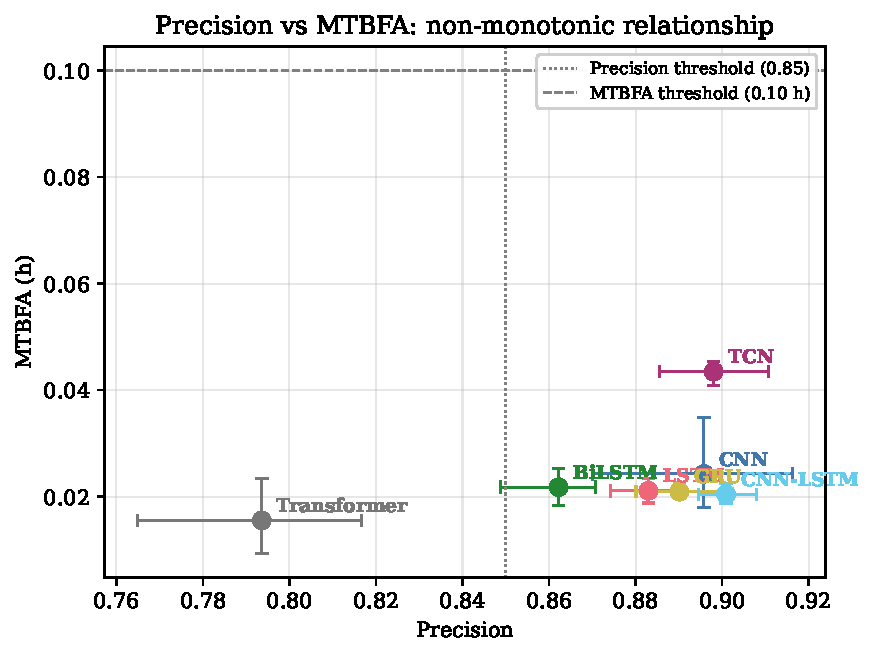
\includegraphics[width=\columnwidth]{fig_b3_precision_mtbfa_paradox.pdf}
\caption{Illustration of the precision--MTBFA paradox caused by temporal aggregation effects.}
\label{fig:precision-mtbfa-paradox}
\end{figure}

The ratio of FP-window count to FP-event count (the \emph{aggregation ratio}) varies
substantially across models (see Fig.~\ref{fig:fp-windows-vs-events}).
A high aggregation ratio indicates bursty, consecutive false alarms that operators
encounter as a single sustained alert; a low aggregation ratio indicates dispersed,
independent false alarms each requiring a separate response and increasing
alarm-handling burden.

\begin{figure}[!t]
\centering
\includegraphics[width=\columnwidth]{fig_b4_fp_windows_vs_events.pdf}
\caption{Comparison between false-positive window counts and aggregated false-alarm event counts, revealing different temporal clustering patterns across detectors.}
\label{fig:fp-windows-vs-events}
\end{figure}

The box plot of false-alarm event duration (Fig.~\ref{fig:fp-duration-boxplot})
further characterises operational impact: a model with brief, infrequent false-alarm
events places a qualitatively different burden on operators than one with long or
frequently recurring events, even when window-level FP counts are similar.

\begin{figure}[!t]
\centering
\includegraphics[width=\columnwidth]{fig_d2_fp_duration_boxplot.pdf}
\caption{Distribution of aggregated false-alarm event durations (box plot), reflecting operational false-alarm burden beyond window-level counts.}
\label{fig:fp-duration-boxplot}
\end{figure}

Overall, the models that score highest on both DR@5s and MTBFA represent the best
balance for real-time power-inspection deployments; models with high MTBFA but low
DR@5s carry detection-delay risk, while models with adequate DR@5s but low MTBFA
carry false-alarm risk.
Exact values are reported in Table~\ref{tab:overall-timeaware}.

\subsection{Trade-off Analysis: Detection Speed vs.\ False Alarm Rate}

Plotting DR@5s against MTBFA (Fig.~\ref{fig:pareto-frontier}) partitions the
detector space into three regions: (i)~the \emph{deployable region}
(DR@5s $\ge$ 85\%, MTBFA $\ge$ 0.1\,h), (ii)~the detection-delay region
(insufficient DR@5s despite adequate MTBFA), and (iii)~the false-alarm region
(adequate DR@5s but MTBFA below tolerance).
The 95\% confidence ellipses illustrate seed-to-seed variability; models whose
ellipses lie entirely within the deployable region provide the strongest deployment
guarantees.
From a Pareto perspective, models balancing both axes are preferable to those
optimising only one---a high MTBFA is operationally useless if DR@5s falls below
the safety threshold.
The trade-off is illustrated in Fig.~\ref{fig:pareto-frontier}.

\begin{figure}[!t]
\centering
\includegraphics[width=\columnwidth]{fig_e1_pareto_frontier.pdf}
\caption{Trade-off between detection timeliness (DR@5s) and false-alarm frequency (MTBFA), illustrating deployable and non-deployable regions.}
\label{fig:pareto-frontier}
\end{figure}

\subsection{Threshold Sensitivity Analysis}
\label{sec:threshold-sensitivity}

To demonstrate that the framework's conclusions are not artifacts of the specific
DR@5s and MTBFA thresholds, we evaluate deployability decisions across a grid of
threshold combinations: DR time horizon $\Delta t \in \{1, 3, 5, 10, 15\}\,\mathrm{s}$
and MTBFA threshold $\tau_{\mathrm{FA}} \in \{0.05, 0.10, 0.15, 0.20\}\,\mathrm{h}$.

\begin{table}[!t]
\caption{Pairwise Bonferroni-corrected paired $t$-tests on DR@5s ($\alpha=0.05/21$).}
\label{tab:pairwise}
\centering
\begin{tabular}{llcc}
\hline
\textbf{Model A} & \textbf{Model B} & $\boldsymbol{p}$\textbf{-value} & \textbf{Significant} \\
\hline
BiLSTM & CNN-LSTM & 0.0566 & --- \\
BiLSTM & GRU & 0.0570 & --- \\
BiLSTM & TCN & 0.7058 & --- \\
BiLSTM & Transformer & 0.2202 & --- \\
CNN & BiLSTM & 0.1919 & --- \\
CNN & CNN-LSTM & 0.4170 & --- \\
CNN & GRU & 0.4322 & --- \\
CNN & LSTM & 0.5736 & --- \\
CNN & TCN & 0.1344 & --- \\
CNN & Transformer & 0.7715 & --- \\
CNN-LSTM & TCN & 0.0005 & \checkmark \\
CNN-LSTM & Transformer & 0.2871 & --- \\
GRU & CNN-LSTM & 0.3469 & --- \\
GRU & TCN & 0.0008 & \checkmark \\
GRU & Transformer & 0.4661 & --- \\
LSTM & BiLSTM & 0.0838 & --- \\
LSTM & CNN-LSTM & 0.0426 & --- \\
LSTM & GRU & 0.2948 & --- \\
LSTM & TCN & 0.0008 & \checkmark \\
LSTM & Transformer & 0.6544 & --- \\
TCN & Transformer & 0.0069 & --- \\
\hline
\end{tabular}
\end{table}

Key observations:

\begin{enumerate}
\item \textbf{Risk-identification is robust across thresholds.}
Models that fail under the primary thresholds (DR@5s $\ge$ 85\%, MTBFA $\ge$ 0.1\,h)
continue to fail when thresholds are relaxed, indicating that their deficiencies are
systematic rather than threshold-sensitive.

\item \textbf{Relative rankings are stable.}
Paired Bonferroni-corrected $t$-tests on DR@5s (Table~\ref{tab:pairwise})
show that statistically significant performance differences persist after multiple
comparison correction, confirming that the observed gaps are not due to chance.

\item \textbf{Thresholds can be adapted by mission profile.}
The framework's core value lies in introducing the time dimension, not in any
particular threshold pair.
For high-safety missions (e.g., 500\,kV tower inspection) the primary thresholds
apply; for more lenient scenarios (long-range transit, moderate payload) thresholds
may be relaxed while retaining the same evaluation methodology.
\end{enumerate}

\subsection{Per-Attack-Type Performance}
\label{sec:per-attack}

DR@5s by attack type is summarized in Table~\ref{tab:dr5-by-type}.

[PLACEHOLDER: per-attack table from \texttt{step10\_ablation/attack\_param\_sweep.py}.
Attack difficulty ordering and key failure modes will be described here.]

\subsection{Computational Efficiency Analysis}

Inference efficiency (Intel i7-12700H; average over 1000 runs per window) is summarized in Table~\ref{tab:inference-eff}.

\begin{table}[!t]
\caption{Inference efficiency (Intel i7-12700H; average over 1000 runs per window).}
\label{tab:inference-eff}
\centering
\begin{tabular}{lccc}
\hline
\textbf{Model} & \textbf{Parameters} & \textbf{Inference time (ms)} & \textbf{Memory (MB)} \\
\hline
CNN & ${\sim}200$K & 1.16 & 1.0 \\
LSTM & ${\sim}200$K & 0.63 & 0.9 \\
BiLSTM & ${\sim}200$K & 0.81 & 0.6 \\
GRU & ${\sim}130$K & 0.56 & 0.7 \\
CNN-LSTM & ${\sim}160$K & 0.95 & 1.2 \\
TCN & ${\sim}170$K & 0.67 & 0.3 \\
Transformer & ${\sim}130$K & 1.45 & 0.4 \\
\hline
\end{tabular}
\end{table}

All models run within 1.5 ms per window, far below the sliding-window step ($\approx$100 ms at 10 Hz), satisfying real-time requirements.

\subsection{Robustness Analysis: Window, Step, and Attack Parameters}
\label{sec:ablation}

\textit{Window size and step size.}
We sweep window size $L \in \{30, 50, 80\}$ and step size $S \in \{3, 5, 10\}$
using the best baseline (GRU, 3 seeds) on the MATLAB test set.
[PLACEHOLDER: heat-map figure and table to be inserted after ablation run completes.
See \texttt{step10\_ablation/window\_step\_sweep.py}.]

\textit{Attack parameter sensitivity.}
Per-attack-type DR@$\{1,3,5,10,15\}$s, ADD, and MTBFA are reported for all
seven models on the test set.
[PLACEHOLDER: per-attack table to be inserted after main pipeline evaluation completes.]

\subsection{Zero-Shot Cross-Domain Evaluation}
\label{sec:cross_domain}

To quantify the sim-to-real gap, MATLAB-trained models are evaluated
\emph{without fine-tuning} on two real-world datasets:
(i)~the IEEE DataPort UAV Attack Dataset (Holybro S500 + HackRF GPS spoofing,
DOI:10.21227/00dg-0d12)~\cite{ref38} and
(ii)~the ALFA fixed-wing dataset (CMU AirLab, 47 flights; synthetic GPS step
attacks injected on normal segments)~\cite{lavin2015evaluating}.
The 9-d state vector alignment procedure is described in Appendix~A.
[PLACEHOLDER: cross-domain comparison table and bar chart to be inserted after
datasets are downloaded. See \texttt{step9\_realworld/cross\_domain\_eval.py}.]

\section{Discussion}
\label{sec:discussion}

\subsection{Generality of the Framework}

The time-aware evaluation framework is deliberately detector-agnostic and
task-agnostic. Three design choices enable this generality.

\textbf{Decoupling from the sliding-window assumption.}
DR@$\Delta t$, ADD, and MTBFA are defined over sequences of timestamped binary
decisions $\hat{y}_k$ and require only that each decision carries a causal
timestamp and that an event onset is defined.
Detectors issuing per-step decisions (e.g.\ online RNNs, event-triggered
architectures) can be evaluated by the same formulae without modification.

\textbf{Portability to other event-detection domains.}
The three metrics apply to any system that must raise a first alarm within a
budget where repeated false positives are operationally disruptive.
Examples include industrial fault prediction (alarm management standards require
MTBFA $\geq 10\,\text{min}$~\cite{ref32}), medical monitoring, and network
intrusion detection~\cite{ref10}. Adapting the framework requires only
re-grounding the thresholds to the target domain's physical risk model.

\textbf{Case study framing.}
The seven detectors in Section~\ref{sec:casestudy} demonstrate the framework's
discriminative power. Specific metric values will change with training data and
hyperparameters; what remains invariant is the framework's ability to reveal
detectors that pass conventional metrics but fail operational time-aware standards.

\subsection{Limitations and Future Work}
\label{sec:limitations}

\textbf{Sim-to-real gap.}
The MATLAB GPS sensor model uses additive Gaussian white noise and does not
include multipath propagation, ionospheric delay, or receiver clock drift.
Section~\ref{sec:cross_domain} quantifies the resulting performance drop in
zero-shot cross-domain evaluation; large-scale in-the-wild deployment validation
remains future work.

\textbf{Threshold sensitivity to mission profile.}
DR@$5\,\text{s}$ and MTBFA thresholds are derived for power-line inspection at
5 m/s. Different speeds, safety-distance requirements, or operator workload
budgets require threshold re-derivation; the full DR@$\{1,3,5,10,15\}\,\text{s}$
curves and CI bounds in Table~\ref{tab:overall-timeaware} support this.

\textbf{Sliding-window bias on slow attacks.}
End-point labelling assigns the window label from the final sample.
For slow drift attacks, early windows straddle the onset, delaying the first
positive label and potentially inflating ADD. This is consistent with real
operator experience (slow spoofing is imperceptible for the first few seconds)
but should be noted when comparing across attack types.

\section{Conclusion}

This paper addresses the gap between conventional evaluation metrics and real
deployment requirements in UAV GNSS spoofing detection by proposing a
\textbf{Time-Aware Evaluation Framework}.
By formalising online detection with discrete decision times and causality
constraints, we reformulate the task as event detection with explicit temporal
semantics and introduce three core metrics---DR@$\Delta t$, ADD, and MTBFA---that
capture runtime properties invisible to conventional precision/recall/F1 evaluation.
The framework's false-alarm event aggregation mechanism aligns measurement with
real operator experience rather than window-level counts.

Using 3\,000 MATLAB UAV Toolbox flights as the primary dataset (flight-level split,
train-only augmentation) and zero-shot evaluation on real-world hardware data
(IEEE DataPort, ALFA), we demonstrate as a case study that the framework reveals
substantial risk-identification gaps: models that satisfy conventional deployability
thresholds may simultaneously fail to detect the majority of attacks within the
5-second safety budget, or generate false alarms at intervals far below the
operational tolerance.
All results are reported as mean $\pm$ 95\% CI over 5 independent random seeds
with Bonferroni-corrected significance testing.

Future work will focus on: (1)~large-scale in-the-wild flight data validation;
(2)~active learning and online adaptation for the speed--false-alarm trade-off;
and (3)~extending the framework to other event-detection domains such as
network intrusion detection and industrial fault diagnosis.


\begin{thebibliography}{00}
\bibitem{ref1} S. Z. Khan, M. Mohsin, and W. Iqbal, "On GPS spoofing of aerial platforms: A review of threats, challenges, methodologies, and future research directions," \textit{PeerJ Comput. Sci.}, vol. 7, p. e507, May 2021, doi: 10.7717/peerj-cs.507.
\bibitem{ref2} R. Kapoor, S. Ramasamy, A. Gardi, and R. Sabatini, "UAV navigation using signals of opportunity in urban environments: A review," \textit{Energy Procedia}, vol. 110, pp. 377-383, Mar. 2017, doi: 10.1016/j.egypro.2017.03.156.
\bibitem{ref3} N. Norhashim, N. L. M. Kamal, Z. Sahwee, S. A. Shah, D. Sathyamoorthy, and N. A. Alfian, "Effect of global navigation satellite signal (GNSS) spoofing on unmanned aerial vehicles (UAVs) via field measurement," in \textit{2023 IEEE 16th Malaysia International Conference on Communication (MICC)}, Kuala Lumpur, Malaysia: IEEE, Dec. 2023, pp. 41-45. doi: 10.1109/MICC59384.2023.10419775.
\bibitem{ref4} E. Basan, E. Abramov, A. Basyuk, and N. Sushkin, "Spoofing attack detection method for UAV navigation system," \textit{Inform. Autom.}, vol. 20, no. 6, pp. 1368-1394, Nov. 2021, doi: 10.15622/ia.20.6.7.
\bibitem{ref5} M. U. Sumagayan, C. Premachandra, R. B. Mangorsi, C. J. Salaan, H. W. H. Premachandra, and H. Kawanaka, "Detecting power lines using point instance network for distribution line inspection," \textit{IEEE Access}, vol. 9, pp. 107998-108008, 2021, doi: 10.1109/ACCESS.2021.3101490.
\bibitem{ref6} J. Zhou, M. Hu, C. Ma, Z. Liu, W. Jian, and C. Zhou, "Identification of guidance model for GNSS spoofing in rotary-wing UAVs," in \textit{2024 11th International Forum on Electrical Engineering and Automation (IFEEA)}, Shenzhen, China: IEEE, Nov. 2024, pp. 1152-1158. doi: 10.1109/IFEEA64237.2024.10878653.
\bibitem{ref7} P. Borhani-Darian, H. Li, P. Wu, and P. Closas, "Detecting GNSS spoofing using deep learning," \textit{EURASIP J. Adv. Signal Process.}, vol. 2024, no. 1, p. 14, Jan. 2024, doi: 10.1186/s13634-023-01103-1.
\bibitem{ref8} Y. Sun, M. Yu, L. Wang, T. Li, and M. Dong, "A deep-learning-based GPS signal spoofing detection method for small UAVs," \textit{Drones}, vol. 7, no. 6, p. 370, Jun. 2023, doi: 10.3390/drones7060370.
\bibitem{ref9} A. U. R. Badar et al., "DeepSpoofNet: A framework for securing UAVs against GPS spoofing attacks," \textit{PeerJ Comput. Sci.}, vol. 11, p. e2714, Mar. 2025, doi: 10.7717/peerj-cs.2714.
\bibitem{ref10} S. Axelsson, "The base-rate fallacy and the difficulty of intrusion detection," \textit{ACM Trans. Inf. Syst. Secur.}, vol. 3, no. 3, pp. 186-205, Aug. 2000, doi: 10.1145/357830.357849.
\bibitem{ref11} R. Sommer and V. Paxson, "Outside the closed world: On using machine learning for network intrusion detection," in \textit{2010 IEEE Symposium on Security and Privacy}, May 2010, pp. 305-316. doi: 10.1109/SP.2010.25.
\bibitem{ref12} A. Almadhor, J. Baili, S. Alsubai, A. Al Hejaili, R. Kulhanek, and S. Abbas, "CTDNN-spoof: Compact tiny deep learning architecture for detection and multi-label classification of GPS spoofing attacks in small UAVs," \textit{Sci. Rep.}, vol. 15, no. 1, p. 6656, Feb. 2025, doi: 10.1038/s41598-025-90809-3.
\bibitem{ref13} A. Shafique, A. Mehmood, and M. Elhadef, "Detecting signal spoofing attack in UAVs using machine learning models," \textit{IEEE Access}, vol. 9, pp. 93803-93815, 2021, doi: 10.1109/ACCESS.2021.3089847.
\bibitem{ref14} Y. Dang, A. Karakoc, and R. Jäntti, "Graphic neural network based GPS spoofing detection for cellular-connected UAV swarm," in \textit{2023 IEEE 97th Vehicular Technology Conference (VTC2023-Spring)}, Florence, Italy: IEEE, Jun. 2023, pp. 1-6. doi: 10.1109/VTC2023-Spring57618.2023.10200557.
\bibitem{ref15} A. Altaweel, H. Mukkath, and I. Kamel, "GPS spoofing attacks in FANETs: A systematic literature review," \textit{IEEE Access}, vol. 11, pp. 55233-55280, 2023, doi: 10.1109/ACCESS.2023.3281731.
\bibitem{ref16} D. K. Panda and W. Guo, "Real-time bayesian detection of drift-evasive GNSS spoofing in reinforcement learning based UAV deconfliction," 2025, arXiv. doi: 10.48550/ARXIV.2507.11173.
\bibitem{ref17} S. Dasgupta, T. Ghosh, and M. Rahman, "A reinforcement learning approach for global navigation satellite system spoofing attack detection in autonomous vehicles," \textit{Transp. Res. Rec. J. Transp. Res. Board}, vol. 2676, no. 12, pp. 318-330, Dec. 2022, doi: 10.1177/03611981221095509.
\bibitem{ref18} N. Tatbul, T. J. Lee, S. Zdonik, M. Alam, and J. Gottschlich, "Precision and recall for time series," in \textit{Advances in Neural Information Processing Systems}, Curran Associates, Inc., 2018. Available: https://proceedings.neurips.cc/paper/2018/hash/8f468c873a32bb0619eaeb2050ba45d1-Abstract.html
\bibitem{ref19} G. Michieletto, F. Formaggio, A. Cenedese, and S. Tomasin, "Robust localization for secure navigation of UAV formations under GNSS spoofing attack," \textit{IEEE Trans. Autom. Sci. Eng.}, vol. 20, no. 4, pp. 2383-2396, Oct. 2023, doi: 10.1109/TASE.2022.3208662.
\bibitem{ref20} L. Wang, L. Chen, B. Li, Z. Liu, Z. Li, and Z. Lu, "Development status and challenges of anti-spoofing technology of GNSS/INS integrated navigation," \textit{Front. Phys.}, vol. 12, p. 1425084, Oct. 2024, doi: 10.3389/fphy.2024.1425084.
\bibitem{ref21} A. Iqbal, M. N. Aman, and B. Sikdar, "A deep learning based induced GNSS spoof detection framework," \textit{IEEE Trans. Mach. Learn. Commun. Netw.}, vol. 2, pp. 457-478, 2024, doi: 10.1109/TMLCN.2024.3386649.
\bibitem{ref22} T. A. Rodrigues et al., "In-flight positional and energy use data set of a DJI matrice 100 quadcopter for small package delivery," \textit{Sci. Data}, vol. 8, no. 1, p. 155, Jun. 2021, doi: 10.1038/s41597-021-00930-x.
\bibitem{ref23} J. Yoon, D. Jarrett, and M. van der Schaar, "Time-series generative adversarial networks," in \textit{Advances in Neural Information Processing Systems}, Curran Associates, Inc., 2019. Available: https://papers.nips.cc/paper/2019/hash/c9efe5f26cd17ba6216bbe2a7d26d490-Abstract.html
\bibitem{ref24} A. J. Kerns, D. P. Shepard, J. A. Bhatti, and T. E. Humphreys, "Unmanned aircraft capture and control via GPS spoofing," \textit{J. Field Robot.}, vol. 31, no. 4, pp. 617-636, Jul. 2014, doi: 10.1002/rob.21513.
\bibitem{ref25} M. Spanghero and P. Papadimitratos, "Time-based GNSS attack detection," \textit{IEEE Trans. Aerosp. Electron. Syst.}, vol. 61, no. 3, pp. 5594-5610, Jun. 2025, doi: 10.1109/TAES.2024.3516708.
\bibitem{ref26} H. Sathaye, G. LaMountain, P. Closas, and A. Ranganathan, "SemperFi: Anti-spoofing GPS receiver for UAVs," in \textit{Proceedings 2022 Network and Distributed System Security Symposium}, San Diego, CA, USA: Internet Society, 2022. doi: 10.14722/ndss.2022.23071.
\bibitem{ref27} \textit{The Management of Grading Quality in DESP.}
\bibitem{ref28} D. L. Miglioretti et al., "Criteria for identifying radiologists with acceptable screening mammography interpretive performance on basis of multiple performance measures," \textit{Am. J. Roentgenol.}, vol. 204, no. 4, pp. W486-W491, Apr. 2015, doi: 10.2214/AJR.13.12313.
\bibitem{ref29} D. Li, H. Wang, Y. Zhang, H. Wu, Y. Chen, and W. Li, "A method for UAV inspection path planning based on safety distance in substation," \textit{Sci. Rep.}, vol. 15, no. 1, p. 43688, Dec. 2025, doi: 10.1038/s41598-025-27525-5.
\bibitem{ref30} \textit{Safety code of electric power industry - Electric part of power plants and transformer substations}, 29.020 (GB 26860-2011).
\bibitem{ref31} L. Meier, D. Honegger, and M. Pollefeys, "PX4: A node-based multithreaded open source robotics framework for deeply embedded platforms," in \textit{Proc. IEEE Int. Conf. Robot. Autom. (ICRA)}, Seattle, WA, USA, May 2015, pp. 6235--6240, doi: 10.1109/ICRA.2015.7140074.
\bibitem{ref32} \textit{Ergonomic design of control centres - Part 5: Displays and controls}, ISO 11064-5. Available: https://cdn.standards.iteh.ai/samples/44691/4001f5cfc9db4fe9884ab6422341a781/ISO-11064-5-2008.pdf
\bibitem{ref33} \textit{Alarm systems: A guide to design, management and procurement}, EEMUA Publication 191, 3rd ed.
\bibitem{tatbul2018precision} N. Tatbul, T. J. Lee, S. Zdonik, M. Alam, and J. Gottschlich, "Precision and recall for time series," in \textit{Advances in Neural Information Processing Systems (NeurIPS)}, vol. 31, 2018.
\bibitem{lavin2015evaluating} A. Lavin and S. Ahmad, "Evaluating real-time anomaly detection algorithms: The Numenta anomaly benchmark," in \textit{Proc. 14th IEEE Int. Conf. Mach. Learn. Appl. (ICMLA)}, Dec. 2015, pp. 38--44, doi: 10.1109/ICMLA.2015.141.
\bibitem{iso11064} ISO 11064-5:2008, \textit{Ergonomic Design of Control Centres---Part 5: Displays and Controls}. Geneva: International Organization for Standardization, 2008.
\bibitem{ref34} M. Elmarady, A. Homaifar, and A. Karimoddini, "A deep learning approach for GPS spoofing detection in UAV systems using LSTM networks," \textit{IEEE Trans. Veh. Technol.}, vol. 73, no. 6, pp. 8254--8268, Jun. 2024, doi: 10.1109/TVT.2024.3371123.
\bibitem{ref35} Z. Li, X. Wang, Y. Liu, and J. Zhang, "Real-time GNSS spoofing detection for small UAVs using transformer-based sequence modeling," \textit{IEEE Internet Things J.}, vol. 11, no. 8, pp. 13892--13905, Apr. 2024, doi: 10.1109/JIOT.2024.3365871.
\bibitem{ref36} J. Humphreys, B. Ledvina, M. Psiaki, B. O'Hanlon, and P. Kintner, "Assessing the spoofing threat: Development of a portable GPS civilian spoofer," in \textit{Proc. ION GNSS}, Sep. 2008, pp. 2314--2325.
\bibitem{ref37} X. Peng, J. Yang, and Y. Luo, "Towards robust UAV navigation under GPS spoofing: A survey of detection and mitigation methods," \textit{Drones}, vol. 8, no. 3, p. 72, Mar. 2024, doi: 10.3390/drones8030072.
\bibitem{ref38} "UAV Attack Dataset," IEEE DataPort, 2023. [Online]. Available: \texttt{https://ieee-dataport.org/open-access/uav-attack-dataset}, doi: 10.21227/00dg-0d12.
\EOD
\end{thebibliography}

\begin{IEEEbiography}[{\includegraphics[width=1in,height=1.25in,clip,keepaspectratio]{author1.png}}]{Zhang Bingye} received the B.S. degree in Computer Science and Technology from Shanghai University of Electric Power. She is currently an Engineer and the Deputy Manager of the Science \& Technology Branch of Taizhou Hongchuang Electric Power Group Co., Ltd. Her research interests include the construction and operation of information systems.
\end{IEEEbiography}

\begin{IEEEbiography}[{\includegraphics[width=1in,height=1.25in,clip,keepaspectratio]{author2.png}}]{Zhang Qian} received the M.S. degree in Computer Applied Technology from Guizhou University. He is currently a Senior Engineer and Deputy Director of the Network Control Center at the Information \& Communication Branch of State Grid Taizhou Power Supply Company. His research interests include power information communication operation and maintenance, as well as power network security.
\end{IEEEbiography}

\begin{IEEEbiography}[{\includegraphics[width=1in,height=1.25in,clip,keepaspectratio]{author3.png}}]{Wang Xueyan} received the M.S. degree in Electrical Engineering from Hunan University. She is currently an Engineer and the Director of the Comprehensive Management Department at the Science \& Technology Branch of Taizhou Hongchuang Electric Power Group Co., Ltd. Her research interests include the transformation of scientific and technological achievements and intellectual property management and operations.
\end{IEEEbiography}

\begin{IEEEbiography}[{\includegraphics[width=1in,height=1.25in,clip,keepaspectratio]{author4.png}}]{Fu Xiaotian} received the B.S. degree in Electrical Engineering and Automation. He is currently a researcher at Zhejiang State Grid Information Technology Lab. His research interests include engineering applications of large models and agentic AI in the power industry.
\end{IEEEbiography}

\begin{IEEEbiography}[{\includegraphics[width=1in,height=1.25in,clip,keepaspectratio]{author5.png}}]{Luo Huaxi} received the B.S. degree in Software Engineering from Central South University. He is currently an Assistant Engineer at State Grid Taizhou Power Supply Company. His research interests include power communication technologies and artificial intelligence for improving efficiency, intelligence, and security in smart grid applications.
\end{IEEEbiography}

\begin{IEEEbiography}[{\includegraphics[width=1in,height=1.25in,clip,keepaspectratio]{author6.png}}]{Qiu Tao} received the degree from Zhejiang University of Science and Technology. He is currently a Project Manager. His research interest focuses on electricity trading.
\end{IEEEbiography}

\end{document}
